%
% A header that lets you compile a chapter by itself, or inside a larger document.
% Adapted from stackoverflow.com/questions/3655454/conditional-import-in-latex
%
%
%Use \inbpdocument and \outbpdocument in your individual files, in place of \begin{document} and \end{document}. In your main file, put in a \def \ismaindoc {} before including or importing anything.
%
% David Duvenaud
% June 2011
% 
% ======================================
%
%


\ifx\ismaindoc\undefined
	\newcommand{\inbpdocument}{
		\def \ismaindoc {}
		% Use this header if we are compiling by ourselves.
		\documentclass[a4paper,11pt,authoryear,index]{common/PhDThesisPSnPDF}
		
%\usepackage{draftwatermark}
%\SetWatermarkLightness{0.95}

% ******************************************************************************
% ****************************** Custom Margin *********************************

% Add `custommargin' in the document class options to use this section
% Set {innerside margin / outerside margin / topmargin / bottom margin}  and
% other page dimensions

\ifsetMargin
\else
    \RequirePackage[left=37mm,right=30mm,top=35mm,bottom=30mm]{geometry}
    \setFancyHdr % To apply fancy header after geometry package is loaded
\fi


%\chead{Unfinished draft}
%\cfoot{\texttt{Unfinished draft - compiled on \today{} at \currenttime}}

% *****************************************************************************
% ******************* Fonts (like different typewriter fonts etc.)*************

% Add `customfont' in the document class option to use this section

\ifsetFont
\else
    % Set your custom font here and use `customfont' in options. Leave empty to
    % load computer modern font (default LaTeX font).  

    \RequirePackage{libertine} 
\fi

% *****************************************************************************
% *************************** Bibliography  and References ********************

%\usepackage{cleveref} %Referencing without need to explicitly state fig /table

% Add `custombib' in the document class option to use this section
\ifsetBib % True, Bibliography option is chosen in class options
\else % If custom bibliography style chosen then load bibstyle here

   \RequirePackage[square, sort, numbers, authoryear]{natbib} % CustomBib

% If you would like to use biblatex for your reference management, as opposed to the default `natbibpackage` pass the option `custombib` in the document class. Comment out the previous line to make sure you don't load the natbib package. Uncomment the following lines and specify the location of references.bib file

% \RequirePackage[backend=biber, style=numeric-comp, citestyle=numeric, sorting=nty, natbib=true]{biblatex}
% \bibliography{References/references} %Location of references.bib only for biblatex

\fi


% changes the default name `Bibliography` -> `References'
\renewcommand{\bibname}{References}


% *****************************************************************************
% *************** Changing the Visual Style of Chapter Headings ***************
% Uncomment the section below. Requires titlesec package.

%\RequirePackage{titlesec}
%\newcommand{\PreContentTitleFormat}{\titleformat{\chapter}[display]{\scshape\Large}
%{\Large\filleft{\chaptertitlename} \Huge\thechapter}
%{1ex}{}
%[\vspace{1ex}\titlerule]}
%\newcommand{\ContentTitleFormat}{\titleformat{\chapter}[display]{\scshape\huge}
%{\Large\filleft{\chaptertitlename} \Huge\thechapter}{1ex}
%{\titlerule\vspace{1ex}\filright}
%[\vspace{1ex}\titlerule]}
%\newcommand{\PostContentTitleFormat}{\PreContentTitleFormat}
%\PreContentTitleFormat


% *****************************************************************************
% **************************** Custom Packages ********************************
% *****************************************************************************


% ************************* Algorithms and Pseudocode **************************

%\usepackage{algpseudocode} 


% ********************Captions and Hyperreferencing / URL **********************

% Captions: This makes captions of figures use a boldfaced small font. 
%\RequirePackage[small,bf]{caption}

\RequirePackage[labelsep=space,tableposition=top]{caption} 
%\renewcommand{\figurename}{Figure} %to support older versions of captions.sty
\captionsetup{labelsep = colon,belowskip=12pt,aboveskip=4pt}

% ************************ Formatting / Footnote *******************************

%\usepackage[perpage]{footmisc} %Range of footnote options 


% ****************************** Line Numbers **********************************

%\RequirePackage{lineno}
%\linenumbers

% ************************** Graphics and figures *****************************

%\usepackage{rotating}
%\usepackage{wrapfig}
%\usepackage{float}
\usepackage{subfig} %note: subfig must be included after the `caption` package. 


% ********************************* Table **************************************

%\usepackage{longtable}
%\usepackage{multicol}
%\usepackage{multirow}
%\usepackage{tabularx}


% ***************************** Math and SI Units ******************************

\usepackage{amsfonts}
\usepackage{amsmath}
\usepackage{amssymb}
%\usepackage{siunitx} % use this package module for SI units


% ******************************************************************************
% ************************* User Defined Commands ******************************
% ******************************************************************************

% *********** To change the name of Table of Contents / LOF and LOT ************

%\renewcommand{\contentsname}{My Table of Contents}
%\renewcommand{\listfigurename}{List of figures}
%\renewcommand{\listtablename}{List of tables}


% ********************** TOC depth and numbering depth *************************

\setcounter{secnumdepth}{2}
\setcounter{tocdepth}{2}

% ******************************* Nomenclature *********************************

% To change the name of the Nomenclature section, uncomment the following line

%\renewcommand{\nomname}{Symbols}


% ********************************* Appendix ***********************************

% The default value of both \appendixtocname and \appendixpagename is `Appendices'. These names can all be changed via: 

%\renewcommand{\appendixtocname}{List of appendices}
%\renewcommand{\appendixname}{Appndx}

		% All my custom preamble stuff.  Shouldn't overlap with anything in official-preamble




% Paths to figure and table directories.
\newcommand{\symmetryfigsdir}{figures/symmetries}
\newcommand{\topologyfiguresdir}{figures/topology}
\newcommand{\infinitefiguresdir}{figures/infinite}
\newcommand{\grammarfiguresdir}{figures/grammar}
\newcommand{\introfigsdir}{figures/intro}
\newcommand{\gplvmfiguresdir}{figures/gplvm}
\newcommand{\warpedfiguresdir}{figures/warped-mixtures}
\newcommand{\deeplimitsfiguresdir}{figures/deep-limits}
\newcommand{\quadraturefigsdir}{figures/quadrature}
\newcommand{\additivefigsdir}{figures/additive}
\newcommand{\decompfigsdir}{figures/decomp}
\newcommand{\examplefigsdir}{figures/worked-example}

\usepackage{bm}  % for warped mixtures - is this necessary?
\usepackage{booktabs}
\usepackage{tabularx}
\usepackage{multirow}
\usepackage{datetime}
\renewcommand{\tabularxcolumn}[1]{>{\arraybackslash}m{#1}}
\usepackage{relsize}
\usepackage{graphicx}
\usepackage{amsmath,amssymb,textcomp}
\usepackage{nicefrac}
\usepackage{amsthm}
\usepackage{tikz}
\usetikzlibrary{arrows}
\usetikzlibrary{calc}
\usepackage{nth}
\usepackage{rotating}
\usepackage{array}
\usepackage{fp}
\usepackage{cleveref}   % Note: this package sometimes causes the page counter to reset.
\crefname{equation}{equation}{equations}
\crefname{figure}{figure}{figures}
%\usepackage{common/sectsty}

% Controls capitalization of all headers
%\usepackage{stringstrings}
%\usepackage[explicit]{titlesec}
%\newcommand\SentenceCase[1]{%
%  \caselower[e]{#1}%
%  \capitalize[q]{\thestring}%
%}
%\titleformat{\section}
%  {\normalfont\Large\bfseries}{\thesection}{1em}{\SentenceCase{#1}\thestring}


%\titleformat{\section} % The normal, unstarred version
%    {\Large\bfseries}{}{2ex}
%    {\thesection. \MakeSentenceCase{#1}}

%\titleformat{name=\section,numberless} % The starred version; note the `numberless` key
%    {\Large\bfseries}{}{2ex}
%    {\MakeSentenceCase{#1}}

\usepackage[hyperpageref]{backref}
% Setup to show (pages 4 and 9) sort of thing in the bibliography - DD
%\def\foo{\hspace{\fill}\mbox{}\linebreak[0]\hspace*{\fill}}
%\def\foo{\parbox{3cm}{\hfill}
%\def\foo{\parbox{3cm}{\hfill}
%\newcommand\foo[1]{{\raggedleft{\hfill{\mbox{\hfill{#1}}}}}}
\newcommand{\comfyfill}[1]{% = Thorsten Donig's \signed
  \unskip\hspace*{0.1em plus 1fill}
  \nolinebreak[3]%
  \hspace*{\fill}\mbox{#1}
  \parfillskip0pt\par
}
\newcommand\foo[1]{{\comfyfill{\mbox{#1}}}}
%\newcommand\foo[1]{{\mbox{#1}}}
\renewcommand*{\backref}[1]{}
\renewcommand*{\backrefalt}[4]{%
\ifcase #1 %
%
\or
\foo{(page #2)}%
\else
\foo{(pages #2)}%
\fi
}

\usepackage{stringstrings}

%\newcommand{\headercase}{\
%\DeclareFieldFormat{titlecase}{\MakeSentenceCase{#1}}


%% For submission, make all render blank.
%%%%%%%%%%%%%%%%%%%%%%%%%%%%%%%%%%%%%%%%%%%%%%%%%%%%%%%%%%
%%%% EDITING HELPER FUNCTIONS  %%%%%%%%%%%%%%%%%%%%%%%%%%%
%%%%%%%%%%%%%%%%%%%%%%%%%%%%%%%%%%%%%%%%%%%%%%%%%%%%%%%%%%

%% NA: needs attention (rough writing whose correctness needs to be verified)
%% TBD: instructions for how to fix a gap ("Describe the propagation by ...")
%% PROBLEM: bug or missing crucial bit 

%% use \fXXX versions of these macros to put additional explanation into a footnote.  
%% The idea is that we don't want to interrupt the flow of the paper or make it 
%% impossible to read because there are a bunch of comments.

%% NA's (and TBDs, those less crucially) should be written so 
%% that they flow with the text.

\definecolor{WowColor}{rgb}{.75,0,.75}
\definecolor{SubtleColor}{rgb}{0,0,.50}

% inline
\newcommand{\NA}[1]{\textcolor{SubtleColor}{ {\tiny \bf ($\star$)} #1}}
\newcommand{\LATER}[1]{\textcolor{SubtleColor}{ {\tiny \bf ($\dagger$)} #1}}
\newcommand{\TBD}[1]{\textcolor{SubtleColor}{ {\tiny \bf (!)} #1}}
\newcommand{\PROBLEM}[1]{\textcolor{WowColor}{ {\bf (!!)} {\bf #1}}}

% as margin notes

\newcounter{margincounter}
\newcommand{\displaycounter}{{\arabic{margincounter}}}
\newcommand{\incdisplaycounter}{{\stepcounter{margincounter}\arabic{margincounter}}}

\newcommand{\fTBD}[1]{\textcolor{SubtleColor}{$\,^{(\incdisplaycounter)}$}\marginpar{\tiny\textcolor{SubtleColor}{ {\tiny $(\displaycounter)$} #1}}}

\newcommand{\fPROBLEM}[1]{\textcolor{WowColor}{$\,^{((\incdisplaycounter))}$}\marginpar{\tiny\textcolor{WowColor}{ {\bf $\mathbf{((\displaycounter))}$} {\bf #1}}}}

\newcommand{\fLATER}[1]{\textcolor{SubtleColor}{$\,^{(\incdisplaycounter\dagger)}$}\marginpar{\tiny\textcolor{SubtleColor}{ {\tiny $(\displaycounter\dagger)$} #1}}}

%\renewcommand{\LATER}[1]{}
%\renewcommand{\fLATER}[1]{}
%\renewcommand{\TBD}[1]{}
%\renewcommand{\fTBD}[1]{}
%\renewcommand{\PROBLEM}[1]{}
%\renewcommand{\fPROBLEM}[1]{}
%\renewcommand{\NA}[1]{}


% HUMBLE WORDS: shown slightly smaller when in normal text
% Thanks to Christian Steinruecken!

% HUMBLE WORDS: shown slightly smaller when in normal text
% Christian Steinruecken
%
\makeatletter%
%\def\@humbleformat#1{{\fontsize{}{1em}\selectfont #1}}
%\def\@humbleformat#1{\textsmaller{#1}}%
\newlength{\nonHumbleHeight}
\def\@humbleformat#1{{\settoheight{\nonHumbleHeight}{#1}\resizebox{!}{0.94\nonHumbleHeight}{#1}}}%
\def\@idxhumbleformat#1{{\relscale{0.95}{#1}}}%
%\def\@humbleformat#1{{#1}}%
\def\declareHumble#1#2{%
  \expandafter\def\csname #1\endcsname{\@humbleformat{#2}}%
  \expandafter\def\csname s#1\endcsname{{#2}}%
  \expandafter\def\csname idx#1\endcsname{{\@idxhumbleformat{#2}}}%
}%
\def\humble#1{\@humbleformat{#1}}%
\def\idxhumble#1{\@idxhumbleformat{#1}}%
\makeatother%

% Convenient indexing for humble abbreviations
\def\humbleindex#1#2{\index{#1@\idxhumble{#1}}}



% TODO: Clean up duplicates
\declareHumble{ANOVA}{ANOVA}
\declareHumble{ARD}{ARD}
\declareHumble{BIC}{BIC}
\declareHumble{BMC}{BMC}
\declareHumble{bq}{BQ}
\declareHumble{CRP}{CRP}
\declareHumble{dirpro}{DP}
\declareHumble{HDMR}{HDMR}
\declareHumble{GAM}{GAM}
\declareHumble{GEM}{GEM}
\declareHumble{GMM}{GMM}
\declareHumble{gplvm}{GP-LVM}
\declareHumble{gpml}{GPML}
\declareHumble{GPML}{GPML}
\declareHumble{gprn}{GPRN}
\declareHumble{gpt}{GP}
\declareHumble{gp}{GP}
\declareHumble{HKL}{HKL}
\declareHumble{HMC}{HMC}
\declareHumble{ibp}{IBP}
\declareHumble{iGMM}{iGMM}
\declareHumble{iwmm}{iWMM}
\declareHumble{kCP}{CP}
\declareHumble{kCW}{CW}
\declareHumble{kC}{C}
\declareHumble{KDE}{KDE}
\declareHumble{kLin}{Lin}
\declareHumble{KPCA}{KPCA}
\declareHumble{kPer}{Per}
\declareHumble{kPerGen}{ZMPer}
\declareHumble{kRQ}{RQ}
\declareHumble{kSE}{SE}
\declareHumble{kWN}{WN}
\declareHumble{Lin}{Lin}
\declareHumble{LBFGS}{L-BFGS}
\declareHumble{LIBSVM}{LIBSVM}
\declareHumble{MAP}{MAP}
\declareHumble{mcmc}{MCMC}
\declareHumble{MKL}{MKL}
\declareHumble{MLP}{MLP}
\declareHumble{MNIST}{MNIST}
\declareHumble{MSE}{MSE}
\declareHumble{OU}{OU}
\declareHumble{Per}{Per}
\declareHumble{RBF}{RBF}
\declareHumble{RMSE}{RMSE}
\declareHumble{RQ}{RQ}
\declareHumble{SBQ}{SBQ}
\declareHumble{seard}{SE-ARD}
\declareHumble{sefull}{SE-\textnormal{full}}
\declareHumble{SEGP}{SE-GP}
\declareHumble{SE}{SE}
\declareHumble{SNR}{SNR}
\declareHumble{SSANOVA}{SS-ANOVA}
\declareHumble{SVM}{SVM}
\declareHumble{UCI}{UCI}
\declareHumble{UMIST}{UMIST}
\declareHumble{vbgplvm}{VB GP-LVM}

\newcommand{\kSig}{\boldsymbol\sigma}

\def\subexpr{{\cal S}}
\def\baseker{{\cal B}}
\def\numWinners{k}

\def\ie{i.e.\ }
\def\eg{e.g.\ }
\def\etc{etc.\ }
\let\oldemptyset\emptyset
%\let\emptyset 0




% Unify notation between neural-net land and GP-land.
\newcommand{\hphi}{h}
\newcommand{\hPhi}{\vh}
\newcommand{\walpha}{w}
\newcommand{\wboldalpha}{\bw}
\newcommand{\wcapalpha}{\vW}
\newcommand{\lengthscale}{w}

\newcommand{\layerindex}{\ell}



\newcommand{\gpdrawbox}[1]{
\setlength\fboxsep{0pt}
\hspace{-0.15in} 
\fbox{
\includegraphics[width=0.464\columnwidth]{\deeplimitsfiguresdir/deep_draws/deep_gp_sample_layer_#1}
}}



\newcommand{\procedurename}{ABCD}
\newcommand{\genText}[1]{{\sf #1}}



\newcommand{\asdf}{$^{\textnormal{th}}$}

\newcommand{\binarysum}{\sum_{\bf{x} \in \{0,1\}^D}}
\newcommand{\expect}{\mathbb{E}}
\newcommand{\expectargs}[2]{\mathbb{E}_{#1} \left[ {#2} \right]}
\newcommand{\var}{\mathbb{V}}
\newcommand{\varianceargs}[2]{\mathbb{V}_{#1} \left[ {#2} \right]}
\newcommand{\cov}{\operatorname{cov}}
\newcommand{\Cov}{\operatorname{Cov}}
\newcommand{\covargs}[2]{\Cov \left[ {#1}, {#2} \right]}
\newcommand{\variance}{\mathbb{V}}
\newcommand{\vecop}[1]{\operatorname{vec} \left( {#1} \right)}

\newcommand{\covarianceargs}[2]{\Cov_{#1} \left[ {#2} \right]}
\newcommand{\colvec}[2]{\left[ \begin{array}{c} {#1} \\ {#2} \end{array} \right]}
\newcommand{\tbtmat}[4]{\left[ \begin{array}{cc} {#1} & {#2} \\ {#3} & {#4} \end{array} \right]}

\newcommand{\acro}[1]{{\humble{#1}}}
%\newcommand{\vect}[1]{\boldsymbol{#1}}
\newcommand{\vect}[1]{{\bf{#1}}}
\newcommand{\mat}[1]{\mathbf{#1}}
\newcommand{\pderiv}[2]{\frac{\partial #1}{\partial #2}}
\newcommand{\npderiv}[2]{\nicefrac{\partial #1}{\partial #2}}

\newcommand{\pha}{^{\phantom{:}}}

\newcommand{\argmin}{\operatornamewithlimits{argmin}}
\newcommand{\argmax}{\operatornamewithlimits{argmax}}

% The following designed for probabilities with long arguments

\newcommand{\Prob}[2]{P\!\left(\,#1\;\middle\vert\;#2\,\right)}
\newcommand{\ProbF}[3]{P\!\left(\,#1\!=\!#2\;\middle\vert\;#3\,\right)}
\newcommand{\p}[2]{p\!\left(#1\middle\vert#2\right)}
\newcommand{\po}[1]{p\!\left(#1\right)}
\newcommand{\pF}[3]{p\!\left(\,#1\!=\!#2\;\middle\vert\;#3\,\right)} 
\newcommand{\mean}[2]{{m}\!\left(#1\middle\vert#2\right)}



\newcommand{\valpha}{\boldsymbol{\alpha}}
\newcommand{\va}{\vect{a}}
\newcommand{\vA}{\vect{A}}
\newcommand{\vB}{\mat{B}}
\newcommand{\vb}{\vect{b}}
\newcommand{\vC}{\mat{C}}
\newcommand{\vc}{\vect{c}}
\newcommand{\vecf}{\boldsymbol{f}}
\newcommand{\vell}{\vect{\ell}}
\newcommand{\vepsilon}{\boldsymbol{\epsilon}}
\newcommand{\veps}{\boldsymbol{\epsilon}}
\newcommand{\ve}{\boldsymbol{\epsilon}}
\newcommand{\vf}{\vecf}
\newcommand{\vg}{\vect{g}}
\newcommand{\vh}{\vect{h}}
\newcommand{\vI}{\mat{I}}
\newcommand{\vK}{\mat{K}}
\newcommand{\vk}{\vect{k}}
\newcommand{\vL}{\mat{L}}
\newcommand{\vl}{\vect{l}}
\newcommand{\vmu}{{\boldsymbol{\mu}}}
\newcommand{\vone}{\vect{1}}
\newcommand{\vphi}{{\boldsymbol{\phi}}}
\newcommand{\vpi}{{\boldsymbol{\pi}}}
\newcommand{\vq}{\vect{q}}
\newcommand{\vR}{\mat{R}}
\newcommand{\vr}{\vect{r}}
\newcommand{\vsigma}{{\boldsymbol{\sigma}}}
\newcommand{\vSigma}{\mat{\Sigma}}
\newcommand{\vS}{\mat{S}}
\newcommand{\vs}{\vect{s}}
\newcommand{\vtheta}{{\boldsymbol{\theta}}}
\newcommand{\vu}{\vect{u}}
\newcommand{\vV}{\mat{V}}
\newcommand{\vW}{\mat{W}}
\newcommand{\vw}{\vect{w}}
\newcommand{\vX}{\mat{X}}
\newcommand{\vx}{\vect{x}}
\newcommand{\vY}{\mat{Y}}
\newcommand{\vy}{\vect{y}}
\newcommand{\vzero}{\vect{0}}
\newcommand{\vZ}{\mat{Z}}
\newcommand{\vz}{\vect{z}}


% deep gp notation
\newcommand{\netweights}{w}
\newcommand{\vnetweights}{\vw}
\newcommand{\mnetweights}{\vW}
\newcommand{\outweights}{\v}
\newcommand{\voutweights}{\vv}
\newcommand{\moutweights}{\vV}

\newcommand{\unitparams}{\v}
\newcommand{\vunitparams}{\vv}
\newcommand{\munitparams}{\vV}


\newcommand{\He}{\mathcal{H}}
\newcommand{\normx}[2]{\left\|#1\right\|_{#2}}
\newcommand{\Hnorm}[1]{\normx{#1}{\He}}
\newcommand{\mmd}{{\rm MMD}}


\newcommand{\mf}{\bar{\vf}}

%\newcommand{\mf}{\mu} %{\bar{\ell}}
\newcommand{\lf}{f} % Likelihood function
\newcommand{\st}{_\star}

% from simpler log-bq writeup
\newcommand{\lftwo}{{\log \ell}}
\newcommand{\mftwo}{{\bar \ell}}
\newcommand{\loggp}{{\log\acro{GP}}}%| \bX, \vy )}}
\newcommand{\loggpdist}{{\acro{GP}(\lftwo)}}%| \vX, \vy )}}


\newcommand{\inv}{^{{\mathsmaller{-1}}}}
\newcommand{\tohalf}{^{{\mathsmaller{\nicefrac{1}{2}}}}}

\newcommand{\Normal}{\mathcal{N}}
\newcommand{\N}[3]{\mathcal{N}\!\left(#1 \middle| #2,#3\right)}
\newcommand{\Nt}[2]{\mathcal{N}\!\left(#1,#2\right)}
\newcommand{\NT}[2]{\mathcal{N}\!\left(#1,#2\right)}
\newcommand{\GPdist}[3]{\mathcal{GP}\!\left(#1 \, \middle| \, #2, #3 \right)}
\newcommand{\GPdisttwo}[2]{\mathcal{GP}\!\left(\, #1, #2 \right)}
\newcommand{\bN}[3]{\mathcal{N}\big(#1 \middle| #2,#3\big)}
\newcommand{\boldN}[3]{\text{\textbf{\mathcal{N}}}\big(#1;#2,#3\big)}
\newcommand{\ones}[1]{\mat{1}_{#1}}
\newcommand{\eye}[1]{\mat{E}_{#1}}
\newcommand{\tra}{^{\mathsf{T}}}
%\newcommand{\tra}{^{\top}}
%\mathsf{T}
\newcommand{\trace}{\operatorname{tr}}
\newcommand{\shift}{\operatorname{shift}}
\renewcommand{\mod}{\operatorname{mod}}
\newcommand{\deq}{:=}
\newcommand{\oneofk}{\operatorname{one-of-k}}
%\newcommand{\degree}{^\circ}

\newcommand{\GPt}[2]{\mathcal{GP}\!\left(#1,#2\right)}
%\newcommand{\GPt}[2]{\gp\!\left(#1,#2\right)}

\DeclareMathOperator{\tr}{tr}
\DeclareMathOperator{\chol}{chol}
\DeclareMathOperator{\diag}{diag}

\newenvironment{narrow}[2]{%
  \begin{list}{}{%
  \setlength{\topsep}{0pt}%
  \setlength{\leftmargin}{#1}%
  \setlength{\rightmargin}{#2}%
  \setlength{\listparindent}{\parindent}%
  \setlength{\itemindent}{\parindent}%
  \setlength{\parsep}{\parskip}}%
\item[]}{\end{list}}



\newcommand{\dist}{\ \sim\ }
\def\given{\,|\,}

% Table stuff
\newcolumntype{C}[1]{>{\centering\let\newline\\\arraybackslash\hspace{0pt}}m{#1}}
\newcolumntype{L}[1]{>{\raggedright\let\newline\\\arraybackslash\hspace{0pt}}m{#1}}
\newcolumntype{R}[1]{>{\raggedleft\let\newline\\\arraybackslash\hspace{0pt}}m{#1}}

\newcommand{\defeq}{\mathrel{:\mkern-0.25mu=}}

\def\ie{i.e.\ }
\def\eg{e.g.\ }
\def\iid{i.i.d.\ }
%\def\simiid{\sim_{\mbox{\tiny iid}}}
\def\simiid{\overset{\mbox{\tiny iid}}{\sim}}
\def\simind{\overset{\mbox{\tiny \textnormal{ind}}}{\sim}}
\def\eqdist{\stackrel{\mbox{\tiny d}}{=}}
%\newcommand{\distas}[1]{\mathbin{\overset{#1}{\kern \z@ \sim}}}
%TODO: fix this - it worked outside the thesis!
\newcommand{\distas}[1]{\mathbin{\overset{#1}{\sim}}}

\def\Reals{\mathbb{R}}

\def\Uniform{\mbox{\rm Uniform}}
\def\Bernoulli{\mbox{\rm Bernoulli}}
\def\GP{\mathcal{GP}}
\def\GPLVM{\mathcal{GP-LVM}}




% Kernel stuff

\def\iva{\vect{\inputVar}}
\def\ivaone{\inputVar}
\def\inputVar{x}
\def\InputVar{X}
\def\InputSpace{\mathcal{X}}
\def\outputVar{y}
\def\OutputSpace{\mathcal{Y}}
\def\function{f}
\def\kernel{k}
\def\KernelMatrix{K}
\def\SumKernel{\sum}
\def\ProductKernel{\prod}
\def\expression{e}
\def\feat{\vh}

\newcommand{\kerntimes}{ \! \times \!}
\newcommand{\kernplus}{ \, + \,}


% Proof stuff
\theoremstyle{plain}
\newtheorem{theorem}{Theorem}[section]
\newtheorem{lemma}[theorem]{Lemma}
\newtheorem{prop}[theorem]{Proposition}
\newtheorem{proposition}{Proposition}
\newtheorem*{cor}{Corollary}

% For infinite bq
\newcommand{\iv}{\theta}
\newcommand{\viv}{\vtheta}

% For intro chapter
\newcommand{\funcval}{\vf(\vX)}
\newcommand{\testpoint}{{\vx^\star}}

\newcommand{\underwrite}[2]{{\underbrace{#1}_{\textnormal{#2}}}}



% For kernel figures
\newcommand{\fhbig}{2cm}%
\newcommand{\fwbig}{3cm}%
\newcommand{\kernpic}[1]{\includegraphics[height=\fhbig,width=\fwbig]{\grammarfiguresdir/structure_examples/#1}}%
\newcommand{\kernpicr}[1]{\rotatebox{90}{\includegraphics[height=\fwbig,width=\fhbig]{\grammarfiguresdir/structure_examples/#1}}}%
\newcommand{\addkernpic}[1]{{\includegraphics[height=\fhbig,width=\fwbig]{\grammarfiguresdir/additive_multi_d/#1}}}%
\newcommand{\largeplus}{\tabbox{{\Large+}}}%
\newcommand{\largeeq}{\tabbox{{\Large=}}}%
\newcommand{\largetimes}{\tabbox{{\Large$\times$}}}%
\newcommand{\fixedx}{$x$ (with $x' = 1$)}%

% for warped mixtures
\newcommand{\CLAS}{\vz}  %cluster assignments
\newcommand{\CLASi}{z} % individual cluster assignments


		% ************************ Thesis Information & Meta-data **********************

%% The title of the thesis
\title{Automating statistical modelling}

%\texorpdfstring is used for PDF metadata. Usage:
%\texorpdfstring{LaTeX_Version}{PDF Version (non-latex)} eg.,
%\texorpdfstring{$sigma$}{sigma}

%% The full name of the author
\author{James Robert Lloyd}

%% Department (eg. Department of Engineering, Maths, Physics)
%\dept{Department of Engineering}

%% University and Crest
\university{University of Cambridge}
\crest{
\includegraphics[width=0.25\textwidth]{misc/University_Crest}}

%% You can redefine the submission text:
% Default as per the University guidelines: This dissertation is submitted for
% the degree of Doctor of Philosophy
%\renewcommand{\submissiontext}{change the default text here if needed}

%% Full title of the Degree 
\degree{Doctor of Philosophy}
 
%% College affiliation (optional)
\college{Trinity College}

%% Submission date
\degreedate{December 2014} 

%% Meta information
\subject{Machine Learning}
\keywords{{LaTeX} {PhD Thesis} {Engineering} {University of Cambridge} {Machine Learning} {Gaussian processes} {Time Series} {Model checking} {Model criticism} {Aldous--Hoover} {Networks}}



		\begin{document}
	}	
	\newcommand{\outbpdocument}[1]{
		% Fake chapters so references aren't broken
		\label{ch:intro}                
		\label{ch:dummy}
		\label{ch:discussion}
		%\bibliographystyle{common/CUEDthesis}
		\bibliographystyle{plainnat}
		\bibliography{references.bib}
		\end{document}
	}	
\else
	%If we're inside another document, no need to re-start the document.
	\ifx\inbpdocument\undefined
		\newcommand{\inbpdocument}{}
		\newcommand{\outbpdocument}[1]{}
	\fi
\fi

\inbpdocument

\chapter{Representing probability distributions of exchangeable arrays}
\label{ch:arrays}

In chapter~\ref{ch:networks} we demonstrated how to characterise probability distributions over objects such as networks or user--item rating matrices.
The key properties that allowed us to characterise these distributions were symmetries in the data, or invariances to the way they are stored.
For networks, we assumed that the ordering of the nodes contained no information.
For user--item data we assumed that the order of both users and items were irrelevant to meaning of the data.

In this chapter we extend these ideas of exchangeability to the full generality of any data that can be stored in a relational database.
This essentially includes every form of data imaginable.
We demonstrate that extensions of the \NA{Aldous--Hoover} theorem to $n$-arrays due to Kallenberg are self strengthening to the case of exchangeable databases.
These new theorems reveal a natural parameter space for data stored in relational databases elucidating how to construct appropriate statistical models for such data.

This chapter is largely based on collaborations with Zoubin Ghahramani, Peter Orbanz and Daniel Roy.
In particular, the theorems presented in this chapter appeared at \NA{BNP} and \NA{NIPS} workshops but without proof.

\section{Introduction}

Relational databases are an extremely common data structure so it is natural to want to perform statistical tasks with such data \eg predicting unobserved data or identifying latent structure.
In particular, network data is rarely encountered in isolation \eg in a social network one will often have access to side information about each user.
To perform a statistical analysis of such data we need to estimate parameters of a probabilistic model, but it is not immediately clear what an appropriate parameter space for such a model is.
The choice of parameter space is important because it indicates the targets of statistical inference and shows where we can share statistical strength between different aspects of the data.

We demonstrate that the weak assumption of an appropriate form of exchangeability can provide a natural parameter space.
%Exchangeability is a reasonable assumption whenever we can faithfully model our data as being a random finite sample from some theoretical infinite population where the order of sampling does not matter.
This form of exchangeability is appropriate when the order of the objects underlying a relational database (\eg users and movies in a database of ratings data) is arbitrary or unimportant.
For example, the left hand side of figure~\ref{fig:exchangeable} shows the same network but with differently labeled nodes.
If the labeling is unimportant, then any probabilistic model of such data should assign them the same probability.

\newpage
Relational data are typically stored in arrays; the right hand side of figure~\ref{fig:exchangeable} shows the corresponding adjacency matrix representations of the networks on the left.
We demonstrate that exchangeability of the objects underlying a relational database can be expressed in terms of array exchangeability.
Prior work on array exchangeability, both theoretical \citep[e.g.][]{Hoover1979, Aldous1981a, Hoover1982, Kallenberg1999a, Diaconis2007, Aldous2010, Austin2012, Choi2012, Wolfe2013} and applied \citep[e.g.][]{Hoff2007a,Roy2009,Lloyd2012}, has focused on single exchangaeble arrays.
We show that the representation theorems for single arrays can be used to derive representations for collections of exchangeable arrays \ie exchangeable databases.

\begin{figure}[t]
\centering
\begin{tabular}{c}
\tiny \begin{tikzpicture}[scale=3]
  \begin{scope}[yshift=0cm]
    \tikzstyle{graph_node}=[circle,minimum size=0.0225\textwidth,inner sep=0pt, fill=camlightblue]
    \def \radius {0.0225\textwidth}
    \begin{scope}[xshift=0cm]
      \foreach \s in {1,...,10}
      {
        \node[draw, graph_node] (N\s) at ({360/10 * (\s - 1) + 90}:\radius) {\s};
      }   
      \path (N2) edge (N6);
      \path (N4) edge (N9);
      \path (N5) edge (N6);
      \path (N5) edge (N8);
      \path (N7) edge (N8);
      \path (N8) edge (N9);
      \path (N8) edge (N10);
      \path (N9) edge (N10);
    \end{scope}
    \begin{scope}[xshift=0.08\textwidth]
      \def \s {1}
      \node[draw, graph_node] (N\s) at ({360/10 * (\s - 1) + 90}:\radius) {2};
      \def \s {2}
      \node[draw, graph_node] (N\s) at ({360/10 * (\s - 1) + 90}:\radius) {7};
      \def \s {3}
      \node[draw, graph_node] (N\s) at ({360/10 * (\s - 1) + 90}:\radius) {6};
      \def \s {4}
      \node[draw, graph_node] (N\s) at ({360/10 * (\s - 1) + 90}:\radius) {5};
      \def \s {5}
      \node[draw, graph_node] (N\s) at ({360/10 * (\s - 1) + 90}:\radius) {3};
      \def \s {6}
      \node[draw, graph_node] (N\s) at ({360/10 * (\s - 1) + 90}:\radius) {1};
      \def \s {7}
      \node[draw, graph_node] (N\s) at ({360/10 * (\s - 1) + 90}:\radius) {10};
      \def \s {8}
      \node[draw, graph_node] (N\s) at ({360/10 * (\s - 1) + 90}:\radius) {8};
      \def \s {9}
      \node[draw, graph_node] (N\s) at ({360/10 * (\s - 1) + 90}:\radius) {4};
      \def \s {10}
      \node[draw, graph_node] (N\s) at ({360/10 * (\s - 1) + 90}:\radius) {9};
      \path (N2) edge (N6);
      \path (N4) edge (N9);
      \path (N5) edge (N6);
      \path (N5) edge (N8);
      \path (N7) edge (N8);
      \path (N8) edge (N9);
      \path (N8) edge (N10);
      \path (N9) edge (N10);
    \end{scope}
    \begin{scope}[xshift=0.04\textwidth]
      \node[inner sep=0,text width=0.13\textwidth, text centered,font=\Huge] (note1) at (0,0) {
         $\equiv$};
    \end{scope}
  \end{scope}
  \begin{scope}[xshift=0.16\textwidth]
    \begin{scope}[xshift=0cm]
      \node [mybox] (box){
        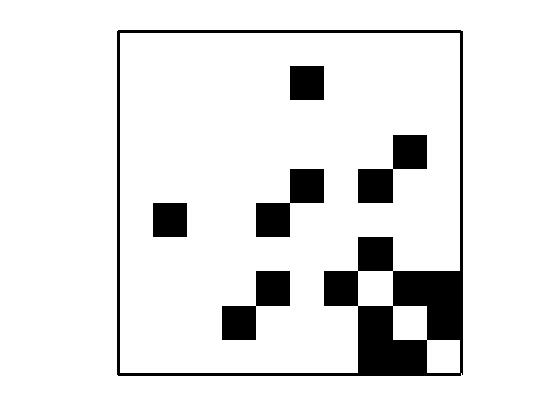
\includegraphics[width=0.225\textwidth]{\arraysfigsdir/adj.png}
      };
    \end{scope}
    \begin{scope}[xshift=0.08\textwidth]
      \node [mybox] (box){
        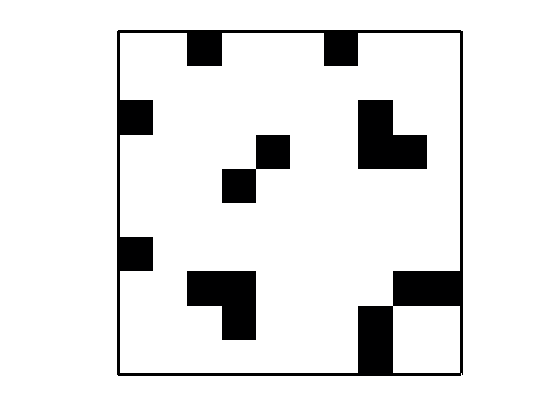
\includegraphics[width=0.225\textwidth]{\arraysfigsdir/adj_perm.png}
      };
    \end{scope}
    \begin{scope}[xshift=0.04\textwidth]
      \node[inner sep=0,text width=0.13\textwidth, text centered,font=\Huge] (note1) at (0,0) {
         $\equiv$};
    \end{scope}
  \end{scope}
\end{tikzpicture}

\end{tabular}
\caption{Left: Networks with equivalent structure but different node labels. Right: Corresponding adjacency matrix representations of these networks}
\label{fig:exchangeable}
\end{figure}

\section{Exchangeable databases}

We abstractly define a database following the entity-relationship formalism \citep[e.g.][]{Ullman2002} where the values of attributes are the result of evaluating a function (relation) over a collection of entities / objects.

\newcommand{\bi}{\bm{i}}
\newcommand{\Types}{T}
\newcommand{\Space}{S}
\begin{definition}[types, signatures, relation]
Fix a finite set $\Types$ of \defn{types}.  Define a \defn{signature} to be a finite sequence $s \in \Types^n$ of types.
Define a \defn{relation $r$ of signature $s \in \Types^n$ with values in a space $\Space$} to be a function from $\Nats^n$ to $\Space$.
\end{definition}

We may encode a relation $r$ with signature $s \in \Types^n$ as an array $X^r \defas (X^r_{\bi})_{\bi \in \Nats^n}$ given by
\[
X^r_{\bi} = r(i_1,\dotsc,i_n), \qquad \text{for } \bi = (i_1,\dotsc, i_n) \in \Nats^n.
\]

\begin{example} 
Let $\Types = \{\textit{users,movies}\}$.  Then a relation $r$ of signature $(\textit{users},\textit{movies})$ taking values in $\{1,2,3,4,5\}$ might store movie ratings with rows corresponding to some enumeration of \textit{users}, and columns corresponding to some enumeration of \textit{movies}.  A relation $r'$ of signature $(\textit{users},\textit{users})$ taking values in $\{0,1\}$ might store the symmetric friendship relations in a social network.
\end{example}

\begin{definition}[database]
Define a \defn{database} to be a collection of $R$ relations $r_1,\dotsc,r_R$ of signature $s_1,\dotsc,s_R$, respectively, taking values in $\Space_1,\dotsc,\Space_R$, respectively.
\end{definition}

We may encode a database as a collection of arrays $(X^{r_j})_{j=1}^R$, where $X^{r_j}$ encodes the relation $r_j$.  
For notational simplicity, we will often refer to the collection of arrays $(X^{r_j})_{j=1}^R$ as if it were the database itself.
%For notational simplicity, we will sometimes write $(X^r)$ to denote such a collection of arrays.

Permuting the ordering of objects within a database results in a permutation of the indices of several of the arrays encoding its relations.  We will now make this precise:
For each type $t \in \Types$, let $p_t \in \SGinf$ be a permutation of $\Nats$. 
Write $p = (p_t ; t \in \Types) \in \SGinf^T$ for the collection of such permutations.
Given a signature $s \in \Types^n$, define $p^s$ to be the map from $\Nats^n$ to $\Nats^n$ such that
\[
p^s(\bi) \defas (p_{s_1}(i_1), \dotsc,p_{s_n}(i_n)), \qquad \text{for } \bi \in \Nats^n.
\]
In other words, $p^s$ maps a sequence $i_1,\dotsc,i_n$ of indices (indexing objects of type $s_1,\dotsc,s_n$, respectively) to the sequence where each index is permuted by the permutation corresponding to its type.

If $X^r$ is the encoding of a relation $r$ with signature $s \in \Types^n$, then the permuted relation $r \circ p$ is represented by the array $X^{r\circ p}$ given by
\[
X^{r \circ p}_{\bi} = X^r_{p^s(\bi)}, \qquad \text{for } \bi \in \Nats^n.
\]

%The permutation of a database $(X^r)$ by $p$ is simply the database $(X^r \circ p)$.

\begin{definition}[exchangeable database]
We say that a random database $(X^{r_j})_{j=1}^R$ is \emph{exchangeable} when it has the same distribution as $(X^{r_j\circ p})_{j=1}^R$ for every $p \in \SGinf^T$.
\end{definition}

%If the ordering of all objects is arbitrary, then $X^r$ is $\pi$-exchangeable where $\pi$ is the partition of consecutive integers with lengths $m^r_1, m^r_2, \ldots, m^r_O$.

%\PROBLEM{Here}

%Let $\Law(Y)$ be the law (distribution) of a random variable $Y$ and define $\chi_m X \defas (X_{i_1\ldots i_d}; \ i_j \le m )$.

The following result characterizes the distribution of any exchangeable database to arbitrary accuracy. 
Let $(\AHvar^t_i)_{i\in\Nats,t \in \Types}$ be a collection of \iid Uniform$[0,1]$ random variables.

\begin{thm}[functional representation for exchangeable databases]
  \label{thm:simple-database}
   Let $(X^{r_j})_{j=1}^R$ be an exchangeable random database.
   Then there exists a sequence of random measurable functions $F^{j,1}, F^{j,2}, \dotsc$ for 
   every $j=1\ldots R$ such that 
   the random databases $(X^{r_j,m})_{j=1}^R$
    converge in distribution to $(X^{r_j})_{j=1\ldots R}$ as $m \to \infty$, where   
%   the sequence of arrays $X^{j,1},X^{j,2},\dotsc$, for $j \in \{1,\dotsc,R\}$, given by
   \[
     X^{r_j,m}_{\bi} := F^{j,m}(\AHvar^{s_j(1)}_{i_1},\dotsc,\AHvar^{s_j(n)}_{i_n}), \qquad \text{for } \bi \in \Nats^n.
   \]
\end{thm}

The proof is based on a reduction to the representation theorem for $\pi$-exchangeable arrays presented in \cite{Kallenberg1999a} but omitted for brevity.

In section

The theorem can be strengthened to state that the law of fixed subarrays are mutually absolutely continuous and the associated Radon-Nikodym derivatives converge uniformly to $1$ as $n \to \infty$.  An almost-sure representational result can also be given at the expense of heavy notation.

%are mutually absolutely continuous for all $m,n \in \Nats$ and the as
%   $\Law((\chi_m X^{j,n})_{j=1\ldots R})$ and $\Law((\chi_m X^{r_j})_{j=1\ldots R})$ are mutually absolutely continuous for all $m,n \in \Nats$ and the associated Radon--Nikodym derivatives converge uniformly to 1 as $n \to \infty$ for fixed $m$.
%\end{thm}

Because the notation is somewhat involved, we present a special case of this theorem applicable to \eg modeling a network with side information for each node.

\begin{cor}
  Consider an exchangeable database with one object type, one unary relationship, and one binary relationship; denote the binary relationship by the array $X=(X_{i,j})_{i,j\in\Nats}$ and the unary relationship with the sequence $C=(C_i)_{i\in\Nats}$.
   Then there exists a sequence of pairs of random measurable functions $(F^n, G^n)_{n\in\Nats}$ and a collection of \iid Uniform$[0,1]$ random variables $(\AHvar_{i})_{i\in\Nats}$ such that if we define the arrays $X^1,X^2,\dotsc$ and sequences $C^1,C^2,\dotsc$ by
   \[ 
     X^n_{i,j} &\defas F^n(\AHvar_{i},\AHvar_{j}), \qquad \text{for } i,j,n\in\Nats, \\
     C^n_{i,j} &\defas G^n(\AHvar_{i}), \qquad \text{for } i,n\in\Nats,
    \]
   then $(X^n,C^n)$ converges in distribution to $(X,C)$ as $n \to \infty$.
   \end{cor}

%\begin{cor}
%  Consider an exchangeable database with one object type, a unary relationship and a binary relationship; denote the binary relationship by the array $(X_{ij})$ and the unary relationship with the sequence $(C_i)$.
%   Then there exists a sequence of pairs of random measurable functions $(F_n, G_n)_{n\in\Nats}$ and a collection of \iid Uniform$[0,1]$ random variables $(\AHvar_{i})_{i\in\Nats}$ such that if we define
%   \begin{equation}
%     ((X_n), (C_n)) := ((F_n(\AHvar_{i},\AHvar_{j}))_{i,j\in\Nats},(G_n(\AHvar_{i}))_{i\in\Nats})
%   \end{equation}
%   then $\Law((\chi_m X_n),(\chi_m C_n)) \textrm{ and } \Law((\chi_m X),(\chi_m C))$ are mutually absolutely continuous for all $m,n \in \Nats$ and the associated Radon--Nikodym derivatives converge uniformly to 1 as $n \to \infty$ for fixed $m$.
%\end{cor}

%\emph{Proof mechanism:}
%
%Each of the arrays $(X^r)$ is $\pi$-exchangeable (see \cite{kallenberg1999multivariate}).
%The collection of arrays can be collected into one larger array (with many duplicated entries) which is still $\pi$-exchangeable.
%We then appeal to theorem 2 of \cite{kallenberg1999multivariate} to get a functional representation of the distribution of the larger array.
%The redundancy of the representation in the larger array can be removed by integrating over the redundant elements.
%These integrals constitute the functions $(F^r_n)$ and the proof concludes by demonstrating the reuqired properties of these functions.\hfill{$\square$}

\begin{rem}[uniform distributions]\label{rem:sym}
The uniform distributions in the theorem are canonical but the theorem still holds with any non-atomic probability measure on a Borel space \eg Gaussian distributions.
\end{rem}
%\begin{rem}[Characteristing the distribution exactly]\label{rem:exact}
%The Aldous--Hoover theorem \cite{Aldous1981a, Hoover1979} for exchangeable arrays demonstrates the existence of functional representations that are equal in distribution to exchanegable arrays.
%A generalisation to exchangeable databases that is analagous to theorem~\ref{thm:simple-database} can be derived but is omitted for brevity since it is significantly more cumbersome to express.
%\end{rem}

\subsection{Intepretation and examples}

Theorem~\ref{thm:simple-database} states that the joint distribution of an exchangeable database can be arbitrarily well approximated by a collection of random measurable functions and uniform random variables.
This functional form provides a set of parameters to be estimated that are naturally hierarchical.
The functions $(F^{j,n})$ capture properties of entire relations whilst the $(U^t_i)$ represent randomness associated with particular objects underlying the relational data.

\subsubsection{Example : Exchangeable networks}

Consider modeling a single binary relation which indicates whether or not two nodes in a network are connected or not.
This data is typically represented in the form of an adjacency matrix $(X_{ij})$ where $X_{ij} = 1$ if and only if node $i$ is connected to node $j$.
Theorem~\ref{thm:simple-database} states that if the distribution of $X$ is exchanegable then it can be arbitrarily well approximated by
\begin{equation}
(F(\AHvar_i, \AHvar_j))
\end{equation}
where $F$ is a random measurable function and $(U_i)$ are \iid Uniform$[0,1]$ random variables.
This special case has been used previously by \cite{Hoff2007a,Roy2009,Lloyd2012} to inspire probabilistic models of networks of the form
\begin{eqnarray}
(\AHvar_i) & \simiid & \textrm{\eg Gaussian} \\
F & \sim & \textrm{\eg Gaussian process, bilinear function}\ldots \\
W_{ij} & := & F(\AHvar_i, \AHvar_j) \\
X_{ij} | W_{ij} & \sim & \textrm{Bernoulli}(\sigma(W_{ij}))\label{eq:graphon}.
\end{eqnarray}
This is demonstrated pictorially in figure~\ref{fig:graphon}; in this case $F$ can be interpreted as a blurred adjacency matrix.

\begin{figure}[ht]
\centering
\begin{tabular}{c}
\begin{tikzpicture}[>=stealth,scale=0.0075\columnwidth]%,transform canvas={xshift=-3cm,yshift=1cm}]
  \begin{scope}[yshift=0.5cm]
  \begin{scope}
    \node [mybox] (box) at (0.5, -0.5){
    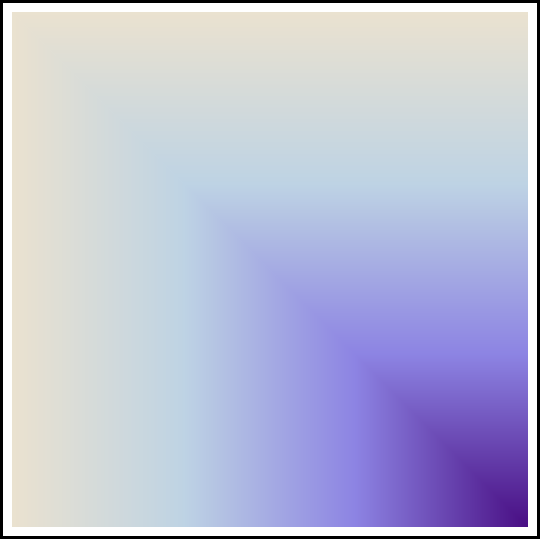
\includegraphics[width=0.225\columnwidth]{\arraysfigsdir/min_function.pdf} 
    };
    %\path[use as bounding box] (-0.5,0.5) rectangle (2.8,-1.5);
    %\draw (0,0) --(0,-1) --(1,-1) --(1,0) --(0,0);
    %\draw (0,0)--(1,-1);
    \node[font=\normalsize] at (0,0.1) {$0$};
    \node[font=\normalsize] at (-0.1,0) {$0$};
    \node[font=\normalsize] at (1,-1.1) {$1$};
    \node[font=\normalsize] at (1.1,-1) {$1$};
    \draw [dashed] (0.2,0.1) -- (0.2,-1.1); \node at (0.2,0.2) {$U_1$};
    \draw [dashed] (-0.1,-0.2) -- (1.1,-0.2); \node at (-0.25,-0.2) {$U_1$};
    \draw [dashed] (0.65,0.1) -- (0.65,-1.1); \node at (0.65,0.2) {$U_2$};
    \draw [dashed] (-0.1,-0.65) -- (1.1,-0.65); \node at (-0.25,-0.65) {$U_2$};
    \node[circle,fill,scale=0.4,color=red] at (0.65,-0.2) {};
  \end{scope}
  \begin{scope}[xshift=2cm]
    \draw (0,0)--(0,-1);
    \draw (-0.05,0)--(0.05,0); \node at (0.15,0) {$0$};
    \draw (-0.05,-1)--(0.05,-1); \node at (0.15,-1) {$1$};
    \node[circle,fill,scale=0.4,color=red] at (0,-0.21) {};
    \node[font=\normalsize] at (0.45,-0.23) {$\mbox{Pr}\lbrace X_{12}=1\rbrace$};
  \end{scope}
  \begin{scope}
  \draw[->] (0.7,-0.25) .. controls (1.3,-0.5) and (1.5,-0.5) .. (1.95,-0.26);
  \draw (1.4,-0.45) node [fill=white] {$\sigma(\Theta)$};
  \end{scope}
  \end{scope}
  %\begin{scope}[xshift=3.4cm]
  %  \node [mybox] (box){
  %  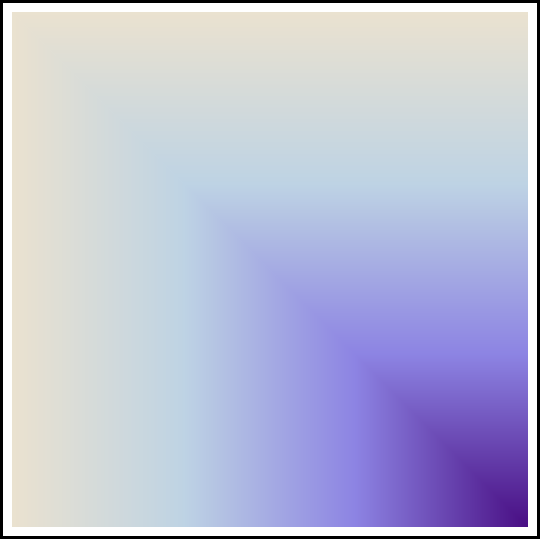
\includegraphics[width=0.18\columnwidth]{\arraysfigsdir/min_function.pdf} 
    %
\includegraphics[width=2.9cm]{\arraysfigsdir/uniform_attachment_graphon.pdf}
  %};
  %\end{scope}  
  %\begin{scope}[xshift=3.4cm]
  \begin{scope}[xshift=-1.2cm]
    \node [mybox] (box){
    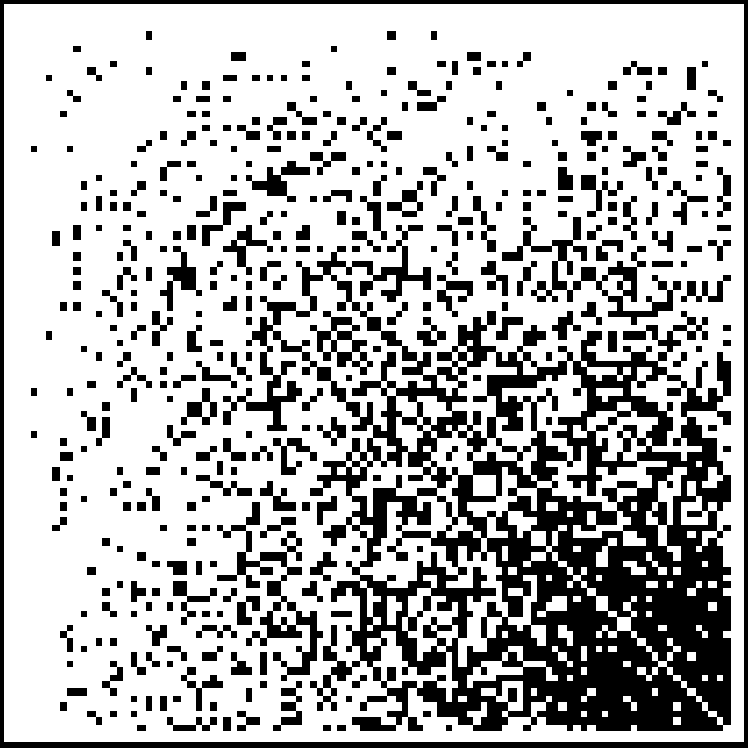
\includegraphics[width=0.225\columnwidth]{\arraysfigsdir/lovasz_sample100.pdf}
    %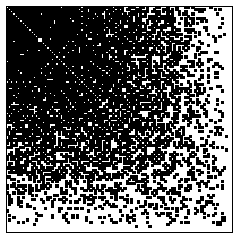
\includegraphics[width=2.8cm]{\arraysfigsdir/uniform_attachment_empirical.pdf}
  };
  \end{scope}
\end{tikzpicture}

\end{tabular}
\caption{
A pictorial representation of a model for network data inspired by the Aldous--Hover representation theorem.
The left shows a random sample of a binary network (represented by an adjacency matrix) generated by a model of the form given by equation~\eqref{eq:graphon}.
This figure is adapted from \cite{Lloyd2012} with permission.}
\label{fig:graphon}
\end{figure}

%\subsubsection{Example : A network with side information}
%
\subsubsection{Example : A simple database}

Consider the simple database shown on the left hand side of figure~\ref{fig:multi-rel-seq}.
There are two objects, students and courses, and three relations, the unary relation `age' acting on students, the binary relation `friends' acting on pairs of students and the binary relation `grade' that acts on students and courses.
Sample data encoded in arrays is shown at the bottom of this figure.

Exchangeability of this database means that the entries of the leftmost table, the rows and columns of the second table and the rows of the third table can be arbitrarily permuted without changing the distribution of the database when viewed as a random variable.
Similarly the columns of the rightmost table may be independently arbitrarily permuted.

The functional form resulting from the application of theorem~\ref{thm:simple-database} to this data structure is shown on the right hand side of figure~\ref{fig:multi-rel-seq}.
The two objects are represented by \iid random variables, $(U_i)$ for students, $(V_i)$ for courses and the three relations are represented by three random functions $F(\AHvar_i),G(\AHvar_i,\AHvar_j)$ and $H(\AHvar_i,\AHvaralt_j)$ whose inputs are the random variables representing the objects the relations act upon.

\begin{figure}[ht]
\centering
\begin{tabular}{cc}
\tiny \begin{tikzpicture}[scale=0.5, node distance = 4cm, auto]
  % Define block styles
  \tikzstyle{decision} = [diamond, draw, fill=blue!20, 
      text width=4.0em, text badly centered, node distance=1.0cm, inner sep=0pt]
  \tikzstyle{invisible} = [diamond, draw=white, fill=white, 
      text width=4.0em, text badly centered, node distance=1.0cm, inner sep=0pt]
  \tikzstyle{block} = [rectangle, draw, fill=blue!20, 
      text width=4.0em, text centered, rounded corners, minimum height=2em]
  \tikzstyle{placeholder} = [rectangle, draw, 
      text width=5em, text centered, rounded corners, minimum height=2em]
  \tikzstyle{line} = [draw, -latex']
  \tikzstyle{cloud} = [draw, ellipse,fill=red!20, node distance=0.75cm,
      minimum height=1em]
  \begin{scope}[yshift=0cm]
    % Place nodes
    \node [block] (student) at (-2.5,1) {Student};
    %\node [block, right of=student] (course) {Course};
    \node [block] (course) at (+2.5,1) {Course};
    \node [decision] at(+2.5, -1.5) (takes) {Takes};
    \node [cloud] (friends) at (-2.5, -4.0) {Friends};
    \node [cloud] (grade) at (+2.5, -4.0) {Grade};
    \node [cloud] (age) at (-5.5, -4.0) {Age};
    % Draw edges
    \path [line] (student) -- (takes);
    \path [line] (course) -- (takes);
    \path [line] (takes) -- (grade);
    %\path [line] (student) -- (observed);
    %\path [line] (observed) -- (friends);
    \draw[->] (student.south) .. controls (-1.0,-1) and (-1.0,-2) .. (friends.north east);
    \draw[->] (student.south) .. controls (-4.0,-1) and (-4.0,-2) .. (friends.north west);
    \path [line] (student.south west) -- (age.north east);
  \end{scope}
  \begin{scope}[yshift=-5cm]
    \draw (-4,0) --(-4,-3) --(-1,-3) --(-1,0) --(-4,0);
    \draw (0,0) --(0,-3) --(5,-3) --(5,0) --(0,0);
    \draw (-6.5,0) --(-6.5,-3) --(-4.5,-3) --(-4.5,0) --(-6.5,0);
    \draw (0,0) --(0,-3) --(5,-3) --(5,0) --(0,0);
    \node at (-3.25, -0.25) {\checkmark};
    \node at (-2.75, -0.25) {\checkmark};
    \node at (-2.25, -0.25) {\checkmark};
    \node at (-1.75, -0.25) {\checkmark};
    \node at (-1.25, -0.25) {\checkmark};
    \node at (-3.75, -0.75) {\checkmark};
    \node at (-3.75, -1.25) {\checkmark};
    \node at (-3.75, -1.75) {\checkmark};
    \node at (-3.75, -2.25) {\checkmark};
    \node at (-3.75, -2.75) {\checkmark};
    \node at (-2.75, -0.75) {$\times$};
    \node at (-3.25, -1.25) {$\times$};
    \node at (-1.25, -1.75) {\checkmark};
    \node at (-2.25, -2.75) {\checkmark};
    
    \node at (0.25, -0.25) {A};
    \node at (4.25, -0.75) {A};
    \node at (3.75, -1.25) {B};
    \node at (1.25, -2.75) {B};
    \node at (0.75, -1.25) {C};
    \node at (2.75, -2.75) {C};
    \node at (2.25, -1.25) {D};
    \node at (2.25, -1.75) {D};
    \node at (3.75, -0.75) {E};
    \node at (4.75, -1.25) {F};
    
    \node at (-5.5, -0.25) {15};
    \node at (-5.5, -0.75) {15};
    \node at (-5.5, -1.25) {15};
    \node at (-5.5, -1.75) {14};
    \node at (-5.5, -2.25) {14};
    \node at (-5.5, -2.75) {16};
  \end{scope}
\end{tikzpicture}
 & \tiny \begin{tikzpicture}[scale=0.5, node distance = 4cm, auto]
  % Define block styles
  \tikzstyle{decision} = [diamond, draw, fill=blue!20, 
      text width=4.0em, text badly centered, node distance=1.0cm, inner sep=0pt]
  \tikzstyle{block} = [rectangle, draw, fill=blue!20, 
      text width=4.0em, text centered, rounded corners, minimum height=2em]
  \tikzstyle{placeholder} = [rectangle, draw, 
      text width=5em, text centered, rounded corners, minimum height=2em]
  \tikzstyle{line} = [draw, -latex']
  \tikzstyle{cloud} = [draw, ellipse,fill=red!20, node distance=0.75cm,
      minimum height=1em]
  \begin{scope}[yshift=0cm]
    % Place nodes
    \node [block] (student) at (-2.5,0) {$(\AHvar_i)$};
    %\node [block, right of=student] (course) {Course};
    \node [block] (course) at (+2.5,0) {$(\AHvaralt_i)$};
    \node [decision, below of=student] (observed) {Observed};
    \node [decision, below of=course] (takes) {Takes};
    \node [cloud] (friends) at (-2.5, -4.0) {Friends};
    \node [cloud] (grade) at (+2.5, -4.0) {Grade};
    \node [cloud] (age) at (-5.5, -4.0) {Age};
    % Draw edges
    \path [line] (student) -- (takes);
    \path [line] (course) -- (takes);
    \path [line] (takes) -- (grade);
    %\path [line] (student) -- (observed);
    \path [line] (observed) -- (friends);
    \draw[->] (student.south) .. controls (-2.0,-0.8) and (-2.0,-1.0) .. (observed.north east);
    \draw[->] (student.south) .. controls (-3.0,-0.8) and (-3.0,-1.0) .. (observed.north west);
    \path [line] (student.south west) -- (age.north east);
  \end{scope}
  \begin{scope}[yshift=-5cm]
    \draw (-4,0) --(-4,-3) --(-1,-3) --(-1,0) --(-4,0);
    \draw (0,0) --(0,-3) --(5,-3) --(5,0) --(0,0);
    \draw (-6.5,0) --(-6.5,-3) --(-4.5,-3) --(-4.5,0) --(-6.5,0);
    \draw (0,0) --(0,-3) --(5,-3) --(5,0) --(0,0);
%    \node at (-3.25, -0.25) {\checkmark};
%    \node at (-2.75, -0.25) {\checkmark};
%    \node at (-2.25, -0.25) {\checkmark};
%    \node at (-1.75, -0.25) {\checkmark};
%    \node at (-1.25, -0.25) {\checkmark};
%    \node at (-3.75, -0.75) {\checkmark};
%    \node at (-3.75, -1.25) {\checkmark};
%    \node at (-3.75, -1.75) {\checkmark};
%    \node at (-3.75, -2.25) {\checkmark};
%    \node at (-3.75, -2.75) {\checkmark};
%    \node at (-2.75, -0.75) {$\times$};
%    \node at (-3.25, -1.25) {$\times$};
%    \node at (-1.25, -1.75) {\checkmark};
%    \node at (-2.25, -2.75) {\checkmark};
    \node at (-2.5, -1.5) {$(G(\AHvar_i, \AHvar_j))$};
    
%    \node at (0.25, -0.25) {A};
%    \node at (4.25, -0.75) {A};
%    \node at (3.75, -1.25) {B};
%    \node at (1.25, -2.75) {B};
%    \node at (0.75, -1.25) {C};
%    \node at (2.75, -2.75) {C};
%    \node at (2.25, -1.25) {D};
%    \node at (2.25, -1.75) {D};
%    \node at (3.75, -0.75) {E};
%    \node at (4.75, -1.25) {F};
    \node at (2.5, -1.5) {$(H(\AHvar_i, \AHvaralt_j))$};
    
%    \node at (-5.5, -0.25) {15};
%    \node at (-5.5, -0.75) {15};
%    \node at (-5.5, -1.25) {15};
%    \node at (-5.5, -1.75) {14};
%    \node at (-5.5, -2.25) {14};
%    \node at (-5.5, -2.75) {16};
    \node at (-5.5, -1.5) {$(F(\AHvar_i))$};
  \end{scope}
\end{tikzpicture}

\end{tabular}
\caption{Left: A pictorial representation of a relational database. Right: The functional representation of the distribution of data of this form guaranteed to be an arbitrarily good approximation by theorem~\ref{thm:simple-database}}
\label{fig:multi-rel-seq}
\end{figure}

%
%\begin{thm}[Kallenberg \cite{kallenberg1999multivariate}]
%\label{theorem:simple}
%Let $\darray$ be an exchangeable array in a Borel space $\dataspace$.  Then there exist some simple exchangeable arrays $X_1,X_2,\dotsc$ such that $\Law(\chi_m X_n) \textrm{ and } \Law(\chi_m X)$ are mutually absolutely continuous for all $m,n \in \Nats$ and the associated Radon--Nikodym derivatives converge uniformly to 1 as $n \to \infty$ for fixed $m$.
%\end{thm}
  
%\emph{Proof sketch:}
%
%Define $M_o := \max_r m^r_o$ and let
%\begin{eqnarray*}
%  (R_{i_1,\ldots,i_{\sum_{o=1}^O M_o}}) & := & (X^1_{i_1,\ldots i_{m^1_1},i_{M_1+1},\ldots,i_{{M_1 + m^1_2}},\ldots,i_{\sum_{o=1}^{O-1}M_o + m^1_O}},\\
%  & & \ldots, \\
%  & & X^R_{i_1,\ldots i_{m^R_1},i_{M_1+1},\ldots,i_{{M_1 + m^R_2}},\ldots,i_{\sum_{o=1}^{O-1}M_o + m^R_O}}).
%\end{eqnarray*}
%R is $\pi$ exchangeable where $\pi$ is the partition of consecutive integers with lengths $M_1, M_2, \ldots, M_O$ so by theorem~\ref{thm:pi-exch}, and a transfer argument there exists a measurable function $f:[0,1]^{\sum_{o=1}^O M_o+1} \to \prod\dataspace^r$ and \iid collection of random variables $(\AHvar_{i}^j)_{i\in\Nats,\,j\in\{1,\ldots,o\}}$, such that
%\[
%R_{i_1,\ldots,i_{\sum_{o=1}^O M_o}} = f(...)\ \as,
%\]
%\NA{and so we do the same integral construction and then prove necessary properties.}\hfill{$\square$}

%\TBD{Give an example with reference to the figure below to show that the theorem isn't really too scary.}

%\section{Exchangeable 2-arrays}
%
%We start by reviewing exchangeability for 2-arrays followed by a corollary applicable to an array with sequential side information (\eg social network and age data).
%
%\begin{definition}
%  A $2$-array $\darray=(\darray_{ij})_{i,j\in\Nats}$ is called a (jointly/weakly) \emph{exchangeable array} if 
%  \begin{equation*}
%    \label{eq:jointly:ex}
%    (\darray_{ij})\eqdist(\darray_{p(i)p(j)}) \qquad\text{ for every } p\in\SGinf\;.
%  \end{equation*}
%\end{definition}
%
%This definition states that the distribution of the array, $\darray$, is invariant to joint permutations of both its rows and columns.
%This assumption would be appropriate for a monopartite graph where the order of the nodes was arbitrary \eg figure~\ref{fig:exchangeable} or a social network.
%
%\subsection{The Aldous--Hoover representation of an exchangeable 2-array}
%
%\begin{thm}[Aldous \cite{Aldous:1981}, Hoover \cite{Hoover1979}]
%  \label{thm:ah}
%  A random 2-array $(\darray_{ij})$ is exchangeable if and only if there exists a measurable function ${f:[0,1]^4\rightarrow\dataspace}$ such that 
%  \begin{equation}
%    (\darray_{ij})\eqdist (f(\AHvar, \AHvar_i,\AHvar_j,\AHvar_{ij})).
%    \label{eq:ah}
%  \end{equation}
%where $\AHvar$, $(\AHvar_i)_{i\in\Nats}$ and $(\AHvar_{ij})_{i\le j\in\Nats}$ are \iid $\Uniform[0,1]$ random variables and $\AHvar_{ji} = \AHvar_{ij}$ for $j < i \in \Nats$.
%\end{thm}
%\begin{rem}[Random function interpretation]\label{rem:rand-func}
%One can alternatively state this theorem by replacing the deterministic function $f(\AHvar, \AHvar_i,\AHvar_j,\AHvar_{ij})$ with a random function $F(\AHvar_i,\AHvar_j,\AHvar_{ij})$.
%This form can be more natural for inspiring models of exchangeable arrays.
%\end{rem}
%\begin{rem}[Uniform priors]\label{remsym}
%The uniform priors in the theorem are canonical but the theorem still holds with any non-atomic probability measure on a Borel space \eg Gaussian distributions.
%\end{rem}
%\begin{rem}[Separately exchangeable arrays]\label{remsep}
%We say that an array $(X_{ij})$ is \emph{separately exchangeable} when $(X_{ij}) \eqdist (X_{p(i)p'(j)})$ for every pair $p,p' \in \SGinf$ of permutations.
%Such symmetry would be appropriate when modeling \eg a user $\times$ movies ratings array.
%A separately exchangeable array can be shown to have the representation $(X_{ij}) \eqdist (f(U,U_i,V_j,W_{ij}))$, where $(U_i)$, $(V_j)$ and $(W_{ij})_{i,j\in\Nats}$ are \iid $\Uniform[0,1]$ random variables.
%\end{rem}
%
%\subsubsection{Interpretation and consequences for statistical modeling}
%
%The Aldous--Hoover representation theorem states that the distribution of any exchanegable array can be modelled using the functional form in equation~\eqref{eq:ah}.
%This equation provides a set of parameters to be estimated that are naturally hierarchical.
%The random variable $\AHvar$ models randomness common to the entire array, the $(U_i)$ represent randomness associated with particular rows and columns and the $(U_{ij})$ model remaining randomness at each entry of the array.
%In the context of a network, $\AHvar$ could model the overall proportion of links, the $(U_i)$ might represent node group structure and the $(U_{ij})$ might capture an observation process.
%
%\subsection{Extension: An array with side information}
%
%We now demonstrate how theorem~\ref{thm:ah} can be used to derive a representation theorem applicable to data that is not naturally represented in the form of a single array.
%For motivation, consider a social network represented by an adjacency matrix $(\darray_{ij})$ together with data on each user represented by a sequence $(\CovData_i)$.
%If the order of users is arbitrary, then any probabilistic model of the combined data should be invariant to \emph{joint} permutations of the rows and volumsn of $\darray$ and the elements of $\CovData$
%In this situation, an appropriate exchangeability assumption for this data is
%\[
%(\darray_{ij},\CovData_i)_{i,j \in \Nats} \eqdist (\darray_{p(i)p(j)}, \CovData_{p(i)})_{i,j\in \Nats}, \textrm{ for every } p\in\SGinf. 
%\]
%
%We know derive a representation theorem for this data.
%Let $U_s$, $s \subseteq \Nats$, be an \iid collection of $\Uniform[0,1]$ random variables.
%For notational simplicity, we will write $U_i \defas U_{\theset i}$, $U_{ij} \defas U_{\theset{i,j}}$, and $U \defas U_\emptyset$.
%
%\begin{cor}
%\label{cor:ahside}
%
%Let $\darray_{ij}$, $i,j\in\Nats$, and $\CovData_i$, $i\in\Nats$, be random variables in $\dataspace$ and $\dataspace'$ respectively.  Then the following are equivalent:
%  
%\begin{enumerate}  
%
%\item[i.] 
%$(\darray_{ij},\CovData_i)_{i,j \in \Nats} \eqdist (\darray_{p(i)p(j)}, \CovData_{p(i)})_{i,j\in \Nats}$, for every $p\in\SGinf$. 
%
%\item[ii.] 
%There are measurable functions $g:[0,1]^4\to\dataspace$ and $h:[0,1]^2\to\dataspace'$ such that 
%   $
%   %\label{eq:ah:cov}
%    (\darray_{ij},\CovData_i)_{i \in \Nats} \eqdist (g(\AHvar,\AHvar_i,\AHvar_j,\AHvar_{ij}), h(\AHvar,\AHvar_i))_{i,j\in\Nats}.
%  $
%
%\end{enumerate}
%\end{cor}
%
%\begin{proof}
%(ii) implies (i) trivially since the collection $\AHvar_s$ is i.i.d.
%Define $(R_{ij}) := (\darray_{ij}, \CovData_i)$, $i,j \in \Nats$, and note that (i) is precisely the statement that $(R_{ij})$ is jointly exchangeable.
%%
%By theorem~\ref{thm:ah}, there exists a measurable function $f:[0,1]^4 \to \dataspace \times \dataspace'$ and \iid collection of random variables $U_s$, $s \subseteq \Nats$, such that $R_{ij} \eqdist f(\AHvar,\AHvar_i,\AHvar_j,\AHvar_{ij}) \, i,j \in \Nats.$
%\[
%R_{ij} \eqdist f(\AHvar,\AHvar_i,\AHvar_j,\AHvar_{ij}) \qquad i,j \in \Nats.
%\]
%In particular, by a transfer argument (see corollary 5.11 of \cite{Kallenberg2002}) there exists $U_s$ such that
%\[
%R_{ij} = f(\AHvar,\AHvar_i,\AHvar_j,\AHvar_{ij})\ \as, \qquad i,j \in \Nats,
%\]
%and so there are measurable functions $f_1,f_2$ into $\dataspace$ and $\dataspace'$, respectively, such that
%\[
%\darray_{ij} = f_1(\AHvar,\AHvar_i,\AHvar_j,\AHvar_{ij}) \ \text{ and } \   % \qquad i,j \in \Nats,
%\]
%and
%\[
%\CovData_i = f_2(\AHvar,\AHvar_i,\AHvar_j,\AHvar_{ij}) \ \as, \qquad i,j \in \Nats.
%\]
%(Indeed, $f_1,f_2$ are just the composition of $f$ and a projection.)
%Define
%\[
%   Z^i_j \defas f_2(\AHvar,\AHvar_i,\AHvar_j,\AHvar_{ij}), \qquad i,j \in \Nats.
%\]
%\fTBD{JRL: I believe this, but for my own education I would like to see a rigorous version of the words `conditioned on'}
%Then conditioned on $\AHvar$ and $\AHvar_i$, the sequence $Z^i_1,Z^i_2,\dotsc$ is \iid and a.s.\ nonrandom and so each element is equal to its expectation
%\[
%h(\AHvar,\AHvar_i) \defas \mathbb{E}[Z^i_1 | \AHvar,\AHvar_i]
%= \int \int f_2(\AHvar, \AHvar_i, x, y)\, \dee x\,\dee y.
%\]
%Taking $g=f_1$ and $h$ satisfies (ii).
%\end{proof}
%
%\section{$d$-arrays, simple arrays and $\pi$-exchangeability}
%
%We now state extensions of the representation theorems to $d$-arrays and more general types of array exchangeabilty.
%The main result of this paper then follows using an analogous proof mechanism to corrolary~\ref{cor:ahside}.
%
%\subsection{Exchangeable $d$-arrays}
%
%\begin{definition}
%  A $d$-array $\darray=(\darray_{i_1\ldots i_d})_{i_j\in\Nats}$ is called a (jointly/weakly) \emph{exchangeable array} if 
%  \begin{equation*}
%    \label{eq:jointly:ex}
%    (\darray_{i_1\ldots i_d})\eqdist(\darray_{p(i_1)\ldots p(i_d)}) \qquad\text{ for every } p\in\SGinf\;.
%  \end{equation*}
%\end{definition}
%
%Aldous--Hoover representations can be derived for $d$-arrays \eg
%
%\begin{thm}[\eg Kallenberg \cite{kallenberg1999multivariate}]
%  \label{theorem:ah3}
%  A random 3-array $(\darray_{ijk})$ is exchangeable if and only if there exists a measurable function ${f:[0,1]^8\rightarrow\dataspace}$ such that 
%  \begin{equation}
%    \label{eq:ah3}
%    (\darray_{ij})\eqdist (f(\AHvar, \AHvar_i,\AHvar_j,\AHvar_k,\AHvar_{ij},\AHvar_{ik},\AHvar_{jk},\AHvar_{ijk})).
%  \end{equation}
%where $\AHvar$, $(\AHvar_i)_{i\in\Nats}$, $(\AHvar_{ij})_{i\le j\in\Nats}$ and $(\AHvar_{ijk})_{i\le j\le k\in\Nats}$ are \iid $\Uniform[0,1]$ random variables.
%\end{thm}
%
%The dimensionality of the domain of the function in equations \ref{eq:ah} and \ref{eq:ah3} grows exponentially with $d$ and thus the representation can become unwieldy quicky.
%To state the general representation therefore requires specialised notation (see proposition 1 of \cite{kallenberg1999multivariate}).
%Fortunately, a simpler representation exists that provides an arbitrarily good approximation to any exchangeable array distribution.
%
%\subsection{Simple arrays}
%
%Call an exchangeable array $(\darray_{i_1\ldots i_d})$ simple if it admits a representation
%\[
%(X_{i_1i_2\ldots i_d}) \eqd (\AHfunction(\AHvar, \AHvar_{i_1},\ldots,\AHvar_{i_d})) \nonumber
%\]
%where $\AHfunction : [0,1]^{d+1} \rightarrow \dataspace$ is a measurable function and $\AHvar$ and $(\AHvar_{i})_{i\in\Nats}$ are \iid $\Uniform[0,1]$ random variables.
%
%Let $\Law(Y)$ be the law (distribution) of a random variable $Y$ and define $\chi_m X \defas (X_{i_1\ldots i_d}; \ i_j \le m )$.
%
%\begin{thm}[Kallenberg \cite{kallenberg1999multivariate}]
%\label{theorem:simple}
%Let $\darray$ be an exchangeable array in a Borel space $\dataspace$.  Then there exist some simple exchangeable arrays $X_1,X_2,\dotsc$ such that $\Law(\chi_m X_n) \textrm{ and } \Law(\chi_m X)$ are mutually absolutely continuous for all $m,n \in \Nats$ and the associated Radon--Nikodym derivatives converge uniformly to 1 as $n \to \infty$ for fixed $m$.
%\end{thm}
%
%For brevity we later denote this type of convergence by $\convdspecial$.
%\TBD{State that this is an arbirarily goos approximation type of result}
%
%\subsection{$\pi$-exchangeability}
%
%In addition to a simplified representation theorem, we will also need a generalised notion of exchangeability \eg
%
%\begin{table}[ht]
%  \centering
%    \begin{tabular}{rclccl}
%      $\darray_{ijk}$ & $\eqd$ & $\darray_{p(i)p(j)p(k)}$ & $\forall\,p\in\SGinf$ & - & Jointly / weakly exchangeable \\
%      $\darray_{ijk}$ & $\eqd$ & $\darray_{p(i)q(j)r(k)}$ & $\forall\,p,q,r\in\SGinf$ & - & Separately / strongly exchangeable \\
%      $\darray_{ijk}$ & $\eqd$ & $\darray_{p(i)q(j)q(k)}$ & $\forall\,p,q\in\SGinf$ & - & A type of $\pi$-exchangeability \\
%    \end{tabular}
%\end{table}
%
%In general, consider a $d$-array, $(X_{i_1i_2\ldots i_d})_{i_j\in\Nats}$, and a partition $\pi$ of the set $\{1,\ldots,d\}$.
%We say that $(X_{i_1i_2\ldots i_d})$ is $\pi$-exchangeable if
%\begin{equation*}
%  (X_{i_1i_2\ldots i_d}) \eqd (X_{p^{\pi_1}(i_1)p^{\pi_2}(i_2)\ldots p^{\pi_d}(i_d)}) \quad \forall\,\,p^1,\ldots,p^{|\pi|}\in\SGinf
%\end{equation*}
%where $\pi_i$ denotes the subset $I \in \pi$ that contains $i$.
%
%The concept of simple arrays applies to $\pi$-exchangeable arrays as well.
%Call a $\pi$-exchangeable array $(\darray_{i_1\ldots i_d})$ simple if it admits a representation
%\[
%(X_{i_1i_2\ldots i_d}) \eqd (\AHfunction(\AHvar_{i_1}^{\pi_1},\ldots,\AHvar_{i_d}^{\pi_d})) \nonumber
%\]
%where $\AHfunction : [0,1]^d \rightarrow \dataspace$ is a random measurable function and $(\AHvar_{i}^j)_{i\in\Nats,\,j\in\{1,\ldots,d\}}$ are \iid $\Uniform[0,1]$ random variables.
%
%\begin{thm}[Kallenberg \cite{kallenberg1999multivariate}]
%\label{thm:pi-exch}
%Let $\darray$ be a $\pi$-exchangeable array in a Borel space $\dataspace$.  Then there exist some simple $\pi$-exchangeable arrays $X_1,X_2,\dotsc$ such that $X_n \convdspecial X$.
%\end{thm}
%
%\subsubsection{Example}
%If $(\darray_{ijk}) \eqd (\darray_{p(i)q(j)q(k)}) \,\, \forall\,p,q\in\SGinf$ then this distribution can be arbitrarily well approximated by $(\AHfunction(\AHvar_i,\AHvaralt_j,\AHvaralt_k))$ where $(\AHvar_i), (\AHvaralt_j)$ are \iid $\Uniform[0,1]$ random variables.
%
%\subsubsection{Relation to full representation theorem}
%
%Show how the simple array representation for a 2-array relates to the full representation theorem \ie either can be interpreted as a sampling distribution in the \iid case or local univariate probability distributions can be encoded into the function representation at very small scales.

\section{Proof of exchangeable database representation theorem}
\label{sec:proof_database}

\section{An almost sure representation theorem}
\label{sec:almost_sure}

\section{A generic generative model}

In analogy to the work of \cite{Hoff2007a, Roy2009, Lloyd2012} on exchangeable arrays, theorem~\ref{thm:simple-database} naturally inspires a generic generative model of exchangeable databases.
Each object in the database is associated with an \iid sample, $\AHvar_i^t$, from some distribution $\mathcal{U}$ \eg Uniform, Gaussian.
For each relation $r_1,\dotsc,r_R$ we independently sample a random function $F^j$ from some distribution $\mathcal{F}^j$, \eg Gaussian process, random (bi/tri/\ldots)linear function.
We denote the evaluation of these functions at the corresponding values of $(\AHvar_i^t)$ by $W^j$.
$W^j$ can then be used to index into a family of observation distribution $L(\cdot)$, \eg Gaussian distributions, to model the value of the relation $r_j$.
\[
(\AHvar_i^t) & \simiid  \mathcal{U} \\
F^r & \sim  \mathcal{F}^r \\
W^j_{\bi} & \defas F^j(\AHvar^{s_j(1)}_{i_1},\cdots,\AHvar^{s_j(n)}_{i_n}) \\
X^{r_j}_{\bi} \given W & \sim  L(W^j_{\bi}) \qquad \text{independently across $j$ and $\bi$.}
\]

\subsection{Prior work using models of this form}

It was demonstrated in \cite{Lloyd2012} that many models of single 2-arrays fit the form of the generic model presented above.
In particular there are models that assume $F$ is linear \citep[e.g.][]{Hoff2007a, Meeds2007, Salakhutdinov2008, Yu2008, Miller2009}, that $F$ is Gaussian process distributed \citep[e.g.][]{Lawrence2009, Yan2011, Lloyd2012} and other non-linear forms for $F$ \citep[e.g.][]{Hoff2002, Roy2009}.
In addition to this there has been a line of work that uses increasingly more expressive forms of the distribution $\mathcal{U}$ \citep[e.g.][]{Wang1987, Nowicki2001, Kemp2006, Xu2006, Meeds2007, Miller2009, Palla2012}.

Many, but not all, of these models have been extended to model $d$-arrays.
A summary of models using linear forms of $F$ is given in \cite{Kolda2009}; non-linear models include \cite{Xu2012}.

For full databases, the literature is limited to clustering models \cite{Kemp2006} and models using linear forms for the $F^r$ \citep[e.g.][]{Acar, Acar2012, Acar2013, Andersen2013, Davison, Ermis1958, Gallinari2011, Jimeng2009, Kong2010, Lippert2008, Networks, Nickel2011, Shangguan2012, Singh, Singha, Singh2008}.

\section{Discussion}

We have demonstrated how the concept of exchangeability can be applied to databases and used to derive a natural parameter space for statistical models of such data.
Identifying a parameter space is the first step in any statistical analysis, allowing either frequentist estimation of the parameters or Bayesian prior specification.
This concept is well established for exchanegable sequences where de Finetti's theorem \citep[e.g.][]{Kallenberg2005} applies.
For exchangeable arrays, the relevant representation theorems were presented by Aldous and Hoover \cite{Aldous1981a, Hoover1979} over 30 years ago but it is only recently that these results are being used to inspire Bayesian models \cite{Hoff2007a, Roy2009, Lloyd2012} and frequentist estimation procedures \cite{Kallenberg1999a,Choi2012, Wolfe2013}.
We hope that this work will continue and be extended to the analysis of exchangeable databases.

\outbpdocument{
\bibliographystyle{plainnat}
\bibliography{references.bib}
}
